\section{Developing and Assessing a Quantitative Evaluation Metric for
Kernel Security}
\label{sec.metric}


In this section, we describe in detail the aforementioned metric to 
quantitatively evaluate kernel security. We first discuss issues with
commonly used metrics for code complexity. Then we present our metric that
focuses on using kernel code paths used by common applications.  We
then show how our metric is able to provide a fair comparison of 
different security systems, their impact on the kernel, 
and to reveal which portions contained fewer bugs.

\subsection{Previous Risk Metrics for Software}

A contributing factor to the kernel security problem is that system
designers 
still lack a standard method for quantifying the safety (or risk) of
privileged code.   \cappos{Is this really true?  No one has ever proposed
a metric?  We do need to do a more detailed analysis of this.  I would vote
to remove this sentence regardless...}

Researchers have studied and explored different metrics to identify and
predict bugs in software systems. 
The number of lines of code has been used as one 
predictor~\cite{Bug-Location}, as has a file's revision status and 
whether or not the file previously contained bugs~\cite{Bug-Location, 
lewis2013does}. Studies have also been done based on 
the number of functions and/or the number of executable lines of code in
the function~\cite{Mining-Metrics}. 
While these metrics can be useful in building models to provide a general
idea about 
where bugs may be located in software systems, they have limitations. 
Firstly, the metrics mentioned above are not specifically designed for
studying bugs in OS kernels. 
\cappos{Why does this matter?}
Therefore, they do not take into account the way system calls are invoked
by user applications. 
Moreover, these metrics can not provide information about the accurate
location of the bugs within the kernel, 
which is important to our study.
\cappos{Are you going to show that this is true?  Can you explain more
about why these do not work?}
\cappos{Do existing metrics work on a LOC level?  }

Without any type of guidance as to what parts of the kernel are safe, past
initiatives, 
such as building a sandbox or using library OSes, could only focus on
isolating user programs.  \cappos{What are you saying?}
These methods can mitigate the problem, but the proposed systems will still
access the kernel the same way as before. 
They simply move the attack surface from between the user space and the
kernel, \yanyan{what's the purpose/consequence of this move? why is this
move good or bad?}
to between these new systems and the kernel, but the surface is not
necessarily reduced. 
As a result, the proposed solutions do not make the systems more secure. 

Recognizing this limitation, we proposed a novel security metric to
quantitatively measure and evaluate the kernel: 
checking kernel coverage safety at the level of lines of code against
existing kernel bugs. 
With this metric, we would be better able to understand security features
of the kernel, 
and design an interface that is exposed to the user space in a secure way.
Ideally, 
this would mean only exposing the safe portions of the kernel to the user
space. 
However, in some cases, risky portions must be exposed to the kernel as
well. 
The kernel coverage safety metric, however, can provide us a guidance 
about the potential dangers and 
can help us safely-reimplement those risky kernel interface (or system
calls) to avoid the potential damage.
%\yanyan{I don't think the new metric alerts us tho. maybe say it provides 
%as a guidance which parts are risky?}




\cappos{end of text}





\subsection{Key Hypothesis}

Our hypothesis is that kernel paths executed by popular applications, 
such as Web browsers, or file editors, are likely to contain fewer
exploitable bugs 
than uncommonly used paths. Our reasoning is that, because they are
frequently used, 
bugs and vulnerabilities in these common kernel paths
would have most likely been caught by developers. 
Note that this does more than indicate which system calls should be used. 
A metric that looks at commonly used kernel paths also excludes odd
execution paths 
through popular system calls. 
This means that the chances to harbor kernel bugs in those commonly used
kernel paths are slim. 

The procedure for testing the hypothesis is described, and the results
discussed, in the following sections. 

\subsection{Foundation for the Metric: Capturing and Evaluating Kernel
Traces}

The first step in proving our hypothesis was to capture the lines of kernel
code executed 
when running applications. The OS kernel code is organized under different
kernel directories. 
Whenever an application tries to access system resources, such as file
system I/O and memory, 
the kernel code under the corresponding paths is executed. Therefore, 
its code execution reflects the basic behavior of the kernel, in response
to user application requests. 
Our metric first identified and captured which lines of code in the kernel
were executed 
when running an user program. We named the resulting captured lines of
code a \textit{kernel trace}. 
A kernel trace is closely related to the program that generated the trace. 
By using the kernel traces, a comparison between different
security systems is possible. 
To capture the kernel trace, we used \texttt{gcov} \cite{gcov}, a program profiling
tool that is a standard utility with the GNU Compiler Collection (GCC) suite. 

The second step was to evaluate security aspects of the kernel traces that
we captured. 
Using the historical kernel vulnerability reports, we collected a list of
severe kernel bugs from 
the National Vulnerability Database, the U.S. government repository of
standards-based \yanyan{what does standards-based mean?}
vulnerability management data \cite{NVD}. We analyzed the bugs as
follows. For each bug, we identified the lines of code 
in the kernel that would trigger it. This can be done by examining 
a patch of the Linux kernel source code to fix the bug. From the patch, 
we can identify \textit{which lines of kernel code need to be modified in order to
remove the bug}. 
A user program that executes the lines of code changed by a patch to fix a
kernel bug is considered to have the \textit{potential to exploit that flaw}.

We determined that the lines of code in the kernel would be risky 
if they triggered one or more kernel vulnerability, and those lines of code 
that did not are considered to be safe. Using the above kernel trace
analysis, 
we empirically labeled the lines of code in the kernel that contain fewer
bugs as safe lines. \yanyan{according to the definition, safe lines should
contain no bug, instead of fewer bugs.}
The safe lines of code would then compose the safe portion of the kernel, 
which can be trusted to build a secure trusted computing base for secure
systems.

\subsection{Verification of Hypothesis}

To verify our hypothesis that commonly used kernel
paths contain fewer bugs, 
we first identified these paths as a subset of the total reachable kernel
paths. These were obtained as follows:

%\begin{enumerate}
First, common paths were captured by running popular user applications. 
We ran applications that are commonly used on a daily basis, such as a Web
browser, file editor, and others. 
In our experiments, we ran Firefox, Chrome, Gedit, and Claws Mail on Native
Linux, 
\cappos{What version of Linux?}  \cappos{Ali: why these apps?}
and performed basic file system operations like open a file, close a file,
make a directory, 
and delete a directory. We ran the experiments 3-4 hours a day for  5 days
in a row.  \cappos{This all needs to be much better explained...}

Next, the total reachable paths were captured by system call fuzzing and
running the Linux kernel test suite. 
We tried to capture the total reachable paths in the kernel as completely
as possible. 
Two approaches were used to capture this trace.

\begin{itemize}
\item First, our system call fuzzing used the Trinity system call fuzz
tester \cite{Trinity}, 
and ran system calls exhaustively with all possible arguments and options. 
We fuzzed more than 300 available system calls, including file management
and network system calls, \yanyan{what is file management?}
which gave us a thorough kernel trace. 

\item In addition, we ran a Linux kernel test suite, 
Linux Test Project (LTP) \cite{LTP} to help capture the total reachable
kernel trace. 
\cappos{Why did we do this?  Was this to validate our results?  Did it work?
Did the test show anything separate from fuzzing?}
Linux Test Project is a mature and well maintained tool to test the Linux
kernel. 
We ran all the available system call test cases with this tool to capture
the kernel trace. 
\end{itemize}
%\end{enumerate}

Combining the kernel traces generated by Trinity and LTP, we were able to
access our total reachable kernel paths.
We found that 38.5\% of the total reachable
kernel paths are commonly used. 
More importantly, only 2.5\% of the bugs examined were found in the common
paths, 
while 50\% of the bugs were found in the total reachable kernel paths. 
Our results confirm that common paths contain fewer bugs than uncommon
paths. \yanyan{I feel this is a bit early to make this conclusion.}

\subsubsection{Coverage Analysis of Common Paths}

The kernel trace coverage of the common paths and the total reachable paths
are shown in Table \ref{table:kernel_coverage}. 
The results show that the size of commonly-used kernel paths is small,
merely 12.4\% of the entire kernel code base. 
The common paths coverage is also significantly smaller than the total
reachable paths coverage 
(about 1/3 of the entire kernel).

It may appear surprising that the total reachable paths coverage is low, 
and accounts for only about one-third of the entire kernel.  However, 
this is consistent with kernel code coverage analysis 
measurements conducted by other researchers \cite{LTP-Coverage}.
One reason that this occurs is that many paths 
in the kernel cannot be accessed from the system call API. Another reason
is that 
while obtaining the kernel coverage data, as most researchers did, we used
a system call fuzzing tool 
and a Linux test suite to generate the kernel trace. The existing fuzzing
tools and test suite do not reach every possible path in the kernel.
\cappos{Why?}

%Although the total reachable paths coverage is not 100\% of the entire
%kernel code base, 
%it is still very large and contains many bugs. 
%However, because the commonly used kernel path coverage is much smaller
%than 
%the total reachable path coverage, this is a positive indication that these
%relatively small areas can be considered safe.

\begin{table}
\centering
\scriptsize
\caption {Kernel Coverage}
\begin{tabular}{|l|c|}
  \hline
  \textbf{Kernel Paths} & \textbf{Kernel Coverage (percentage)} \\
  \hline \hline
  Common Paths & 12.4\% \\
  \hline
  Total Reachable Paths & 32.2\% \\
  \hline
\end{tabular}
\label{table:kernel_coverage}
\end{table}

The results from Figure \ref{fig:subset} and Figure
\ref{fig:key_paths_trace}  \cappos{What do these actually mean?}
show that the common paths are a subset of the
total reachable paths, 
shown by the ``OverlappedLines'' in Figure \ref{fig:subset} and Figure
\ref{fig:key_paths_trace}. 
We closely examined the kernel trace derived from common paths
and the total reachable paths. We found that for each different path
in the kernel, the lines of code 
in the common paths trace also appeared in the total reachable paths trace.
But there are many lines of code (more than 50\%) 
in the total reachable paths trace that are not in the common paths. This
shows that the common paths trace and 
the total reachable paths we obtained are correct, because common paths in
the kernel should definitely be reachable. \yanyan{how to define correct?}
One further finding is that the common paths account
for only 38.5\% of the total reachable paths. 
This suggests that a large portion (61.5\%) of the kernel is not frequently
used by popular applications on a daily basis.

\begin{figure}
\centering
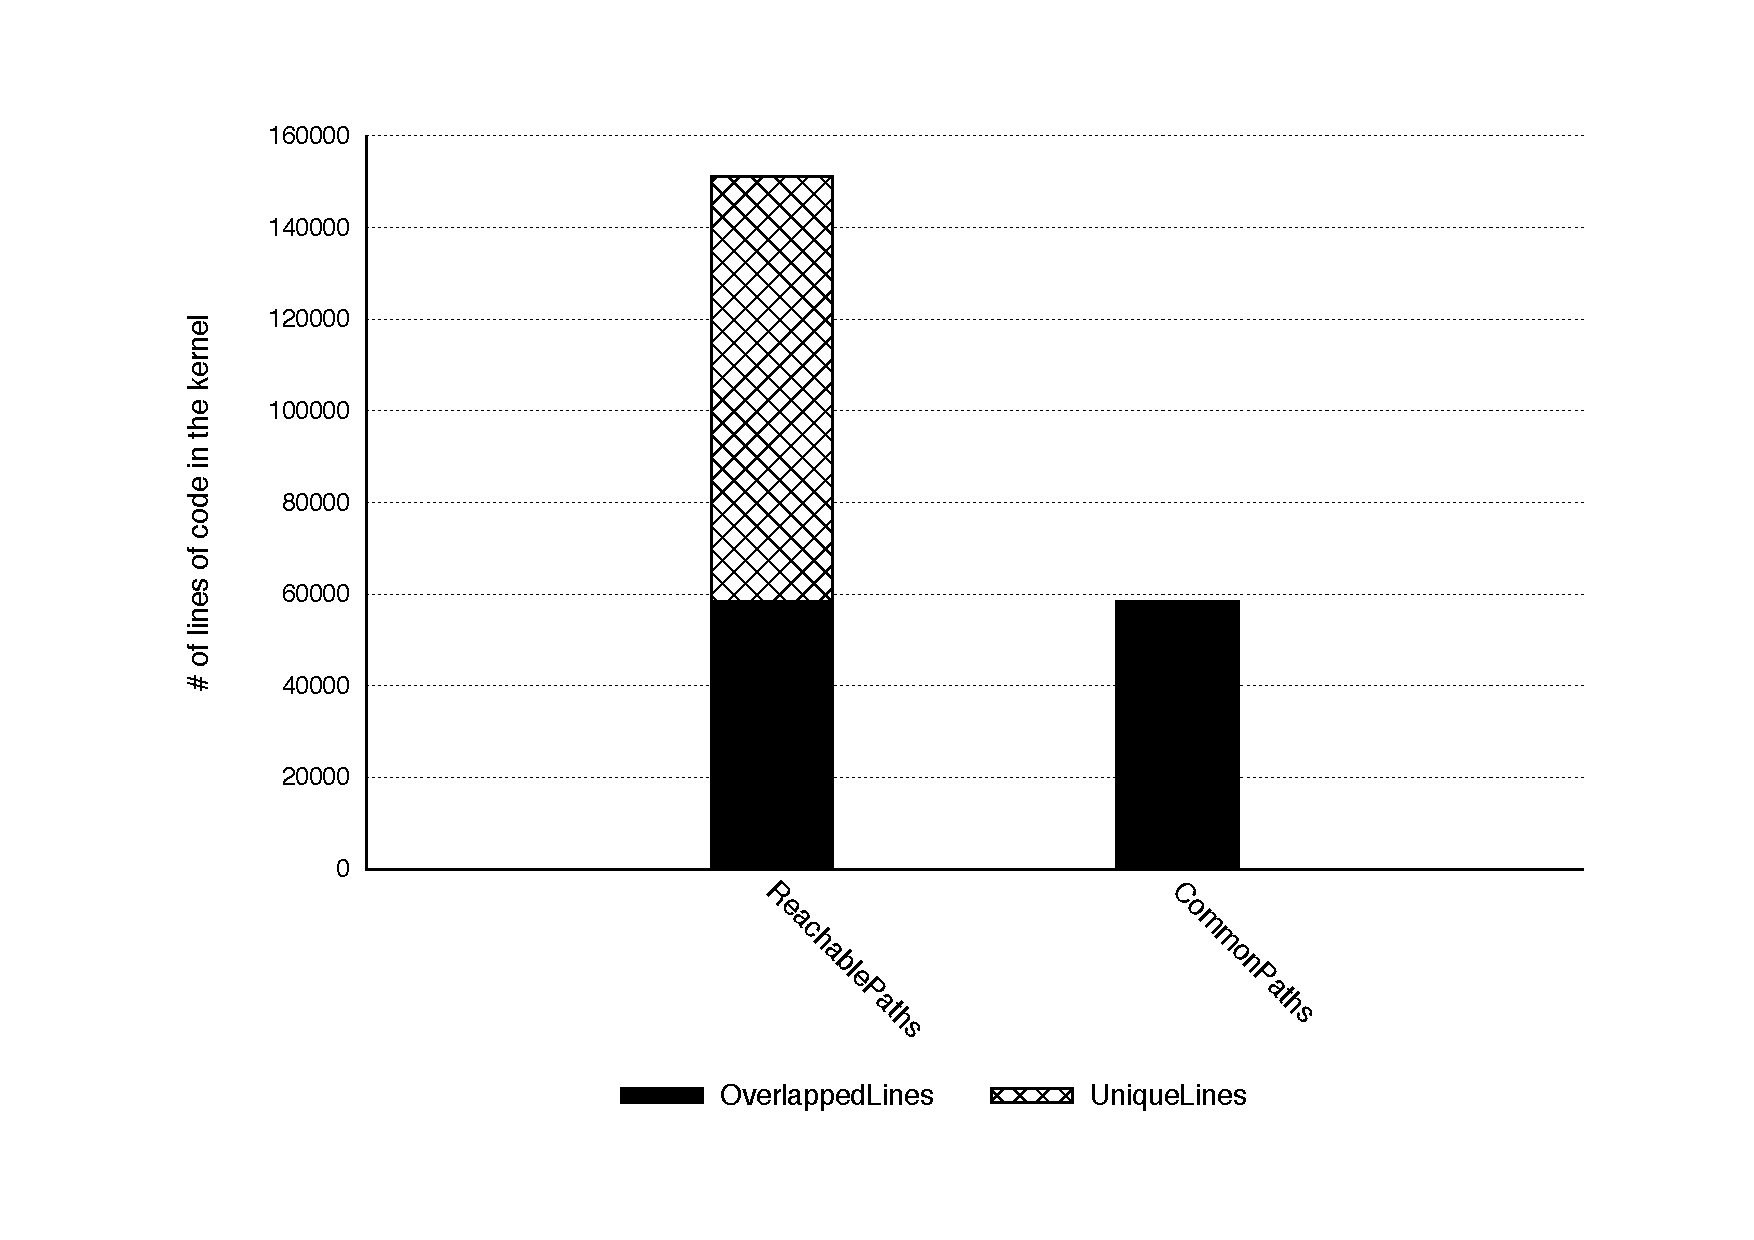
\includegraphics[width=1.0\columnwidth]{diagram/lind_oakland16_diagram_01.pdf}
\caption{Kernel Trace Comparison: Common Paths as a Subset of Reachable
Paths}
\label{fig:subset}
\end{figure}

\begin{figure}
\centering
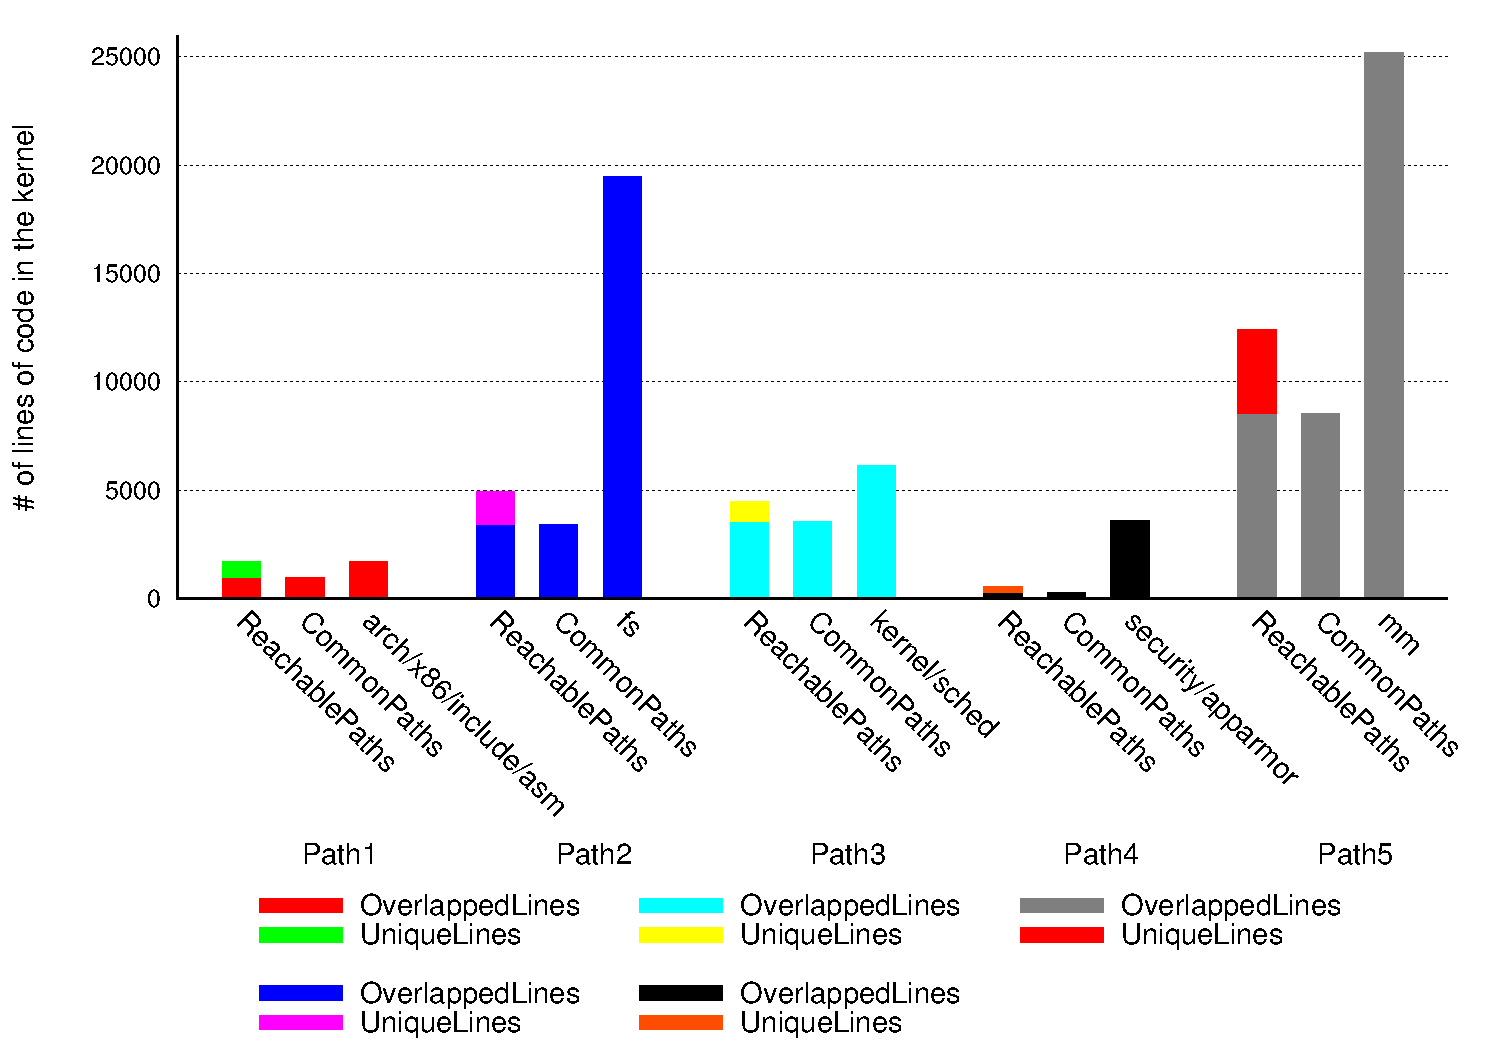
\includegraphics[width=1.0\columnwidth]{diagram/lind_oakland16_diagram_02.pdf}
\caption{Kernel Trace in Key Paths}
\label{fig:key_paths_trace}
\end{figure}

\subsubsection{Security Analysis of Kernel Paths\textendash Locating the
Risky Portions}

To verify our hypothesis, we next checked which portions of
the kernel contained kernel bugs. We examined 40 severe Linux kernel
bugs that had been discovered by the research community in the last five
years (the first two columns in Table 
\ref{table:vulnerabilities_commonly_used_kernel_paths}). 
We used these kernel bugs to check if vulnerabilities existed in certain
kernel traces.   \cappos{How?}
The results of our experiment are shown the last two columns in Table
\ref{table:vulnerabilities_commonly_used_kernel_paths}.

\begin{table*}[!ht]
\scriptsize
\centering
\caption {Linux Kernel Bugs, and Vulnerabilities in Different Portions of
the Kernel 
({\color{red}\ding{51}}: vulnerability in paths; \ding{55}: vulnerability
not in paths)}
\begin{tabular}{|l|l|c|c|}\hline
\multirow{2}{*}{\textbf{Vulnerability}} & \multirow{2}{*}{\textbf{Specific
Type}} & \multicolumn{2}{c|}{\bf Portion of the Kernel} \\
\cline{3-4}
&  & \textbf{Total Reachable Paths} &  \textbf{Common Paths} \\ \hline

 CVE-2014-9529 & concurrency, race condition & {\color{red}\ding{51}} &
\ding{55} \\
 CVE-2014-3631 & NULL pointer dereference & {\color{red}\ding{51}} &
\ding{55} \\
 CVE-2012-6657 & network socket variable mischeck & {\color{red}\ding{51}}
& \ding{55} \\
 CVE-2014-5207 & privilege escalation & \ding{55} & \ding{55} \\
 CVE-2014-5206 & privilege escalation & \ding{55} & \ding{55} \\
 CVE-2014-3153 & privilege escalation & \ding{55} & \ding{55} \\
 CVE-2014-2851 & privilege escalation & \ding{55} & \ding{55} \\
 CVE-2014-2706 & race condition, DoS & {\color{red}\ding{51}} & \ding{55}
\\
 CVE-2014-0100 & race condition, DoS & {\color{red}\ding{51}} & \ding{55}
\\
 CVE-2014-0049 & buffer overflow & \ding{55} & \ding{55} \\
 CVE-2012-6638 & DoS & {\color{red}\ding{51}} & \ding{55} \\
 CVE-2014-0038 & privilege escalation & \ding{55} & \ding{55} \\
 CVE-2013-6368 & privilege escalation & \ding{55} & \ding{55} \\
 CVE-2013-4587 & index error, privilege escalation & \ding{55} & \ding{55}
\\
 CVE-2013-4563 & size/boundary check, DoS & {\color{red}\ding{51}} &
\ding{55} \\
 CVE-2013-4348 & value validation error & \ding{55} & \ding{55} \\
 CVE-2013-4300 & privilege escalation & {\color{red}\ding{51}} & \ding{55}
\\
 CVE-2013-1943 & privilege escalation & \ding{55} & \ding{55} \\
 CVE-2013-2094 & privilege escalation & {\color{red}\ding{51}} & \ding{55}
\\
 CVE-2013-3301 & NULL pointer dereference, DoS & {\color{red}\ding{51}} &
\ding{55} \\
 CVE-2013-1858 & privilege escalation & {\color{red}\ding{51}} & \ding{55}
\\
 CVE-2013-1797 & use-after-free & {\color{red}\ding{51}} & \ding{55} \\
 CVE-2013-1763 & privilege escalation, index error & \ding{55} & \ding{55}
\\
 CVE-2013-0310 & NULL pointer dereference & \ding{55} & \ding{55} \\
 CVE-2012-2136 & heap-based buffer overflow & \ding{55} & \ding{55} \\
 CVE-2012-2100 & lack of sanity check  & \ding{55} & \ding{55} \\
 CVE-2012-0028 & privilege escalation & {\color{red}\ding{51}} & \ding{55}
\\
 CVE-2011-2517 & privilege escalation, buffer overflow &
{\color{red}\ding{51}} & \ding{55} \\
 CVE-2012-2123 & privilege escalation  & {\color{red}\ding{51}} & \ding{55}
\\
 CVE-2012-1146 & NULL pointer dereference  & \ding{55} & \ding{55} \\
 CVE-2012-0207 & divide-by-zero error and panic & \ding{55} & \ding{55} \\
 CVE-2011-2525 & NULL pointer dereference  & {\color{red}\ding{51}} &
\ding{55} \\
 CVE-2011-1076 & NULL pointer dereference  & {\color{red}\ding{51}} &
\ding{55} \\
 CVE-2011-2184 & NULL pointer dereference, none initialization & \ding{55}
& \ding{55} \\
 CVE-2010-2478 & integer overflow & {\color{red}\ding{51}} & \ding{55} \\
 CVE-2010-2960 & NULL pointer dereference  & \ding{55} & \ding{55} \\
 CVE-2010-2492 & privilege escalation, buffer overflow & \ding{55} &
\ding{55} \\
 CVE-2010-2240 & stack overflow & {\color{red}\ding{51}} &
{\color{red}\ding{51}}\\
 CVE-2010-1188 & use-after-free & \ding{55} & \ding{55} \\
 CVE-2010-0437 & NULL pointer dereference  & {\color{red}\ding{51}} &
\ding{55} \\ \hline
 \multicolumn{2}{|c|}{\bf Percentage contains bugs} & {\bf $50\%$} & {\bf
$2.5\%$} \\ \hline
\end{tabular}
\label{table:vulnerabilities_commonly_used_kernel_paths}
\end{table*}

From the results, we can see that commonly used kernel paths contain only
2.5\% of the bugs we had targeted. 
Since the total reachable kernel paths contain 50\% of the bugs we
examined, 
our results show that commonly used kernel paths clearly contain fewer bugs
than other portions of the kernel. 
\cappos{Why?}
Our hypothesis and findings provide insights and guidelines for new designs
of secure systems, 
which will be discussed in the next section. 
\cappos{Is this statistically significant?}




